\section{Numerical Experiments}
In this section, we present convergence analysis results of the Finite Element Method applied to the one-dimensional heat equation. We then compare the computational time of the direct LU-factorization and the iterative CGD and PCGD methods. Afterwards, we present some results of our numerical methods applied to the two-dimensional heat equation. Finally, we present a finance application, namely European options pricing results. 
\subsection{The 1D Fractional Heat Equation - Convergence Results} 
Consider the 1D fractional heat equation on the unit interval \truncdom=$(0,1)$,
\begin{equation} \label{frac_heat_1D}
\begin{split} % \begin{split}
\partial_tu(t,x) + (-\partial_{xx})^{\beta} u(t,x) = 0&, \quad  (t,x)\in(0,T]\times\truncdom, \\
u(0,x) = x(1-x)&, \quad x\in \truncdom, \\ 
u(t,0) = u(t,1) = 0&, \quad t \in [0,T].
\end{split}
\end{equation}
For $T=1$, we apply the finite element method to \eqref{frac_heat_1D} with different combinations of the parameters $\beta$ and $\theta$. Namely we let $\beta\in\{1/4, 1/2, 3/4, 1\}$, and $\theta \in \{0,1/4,1/2,3/4,1\}$ for the $\theta$-scheme time stepping. The discrete equation \eqref{full_disc} will then satisfy $\mathbf{A} =0, \tilde{a}\equiv1$ and $\tilde{\fullstiff} = \mass\sinc\stiff$. \\
\newline
For the error analysis, in \eqref{Refinement1D} we implement a C++ class \lstinline{meshUniformRefinement} that describes the mesh hierarchy used to conduct the convergence analysis. 
\begin{lstlisting}[caption={1D uniform refinement.}, label={Refinement1D}]
class meshUniformRefinement{ 
  public: 
    meshUniformRefinement(size_t N_0, size_t numOfLevels){ 
    h_.resize(numOfLevels); 
	N_dofs_.resize(numOfLevels); 
	meshes_.resize(numOfLevels);
	std::vector<double> L(numOfLevels); 
	std::iota(L.begin(), L.end(), 0); /// Refinement levels
	/// mesh sizes: 1/N0 * 2^{-L}
	std::transform(L.begin(), L.end(), h_.begin(), [&](double level){
	    return 1.0/N_0 * std::pow(2,-level);} );	
        /// Total number of nodes: 1+N0*2^{L}
	std::transform(L.begin(), L.end(), N_dofs_.begin(), [&](double level){
	    return 1 + N_0 * std::pow(2,level);} );
	std::transform(N_dofs_.begin(), N_dofs_.end(), meshes_.begin(), [&](size_t Ndofs){
    	    return Eigen::VectorXd::LinSpaced(Ndofs, 0, 1); } ); 
      }
      
      /// Returns a pointer to the mesh at a given level 
      std::shared_ptr<Eigen::VectorXd> getMesh(size_t level){
	  return std::make_shared<Eigen::VectorXd>(meshes_.at(level));
	}
    std::vector<double> h_; 
    std::vector<size_t> N_dofs_; 
   
  private: 
    std::vector<Eigen::VectorXd> meshes_; 
};
\end{lstlisting}
More precisely, given \lstinline{N_0} and \lstinline{numOfLevels} which defines the number of elements on the coarsest mesh and the number of levels in the mesh hierarchy, respectively, the constructor \lstinline{meshUniformRefinement(size_t N_0, size_t numOfLevels)} constucts the meshes at all levels by uniform refinement, where the number of nodes at each level is given by $1+N_02^{L}$, and the mesh size is given by $1/N_02^{-L}$ where $L\in\{0,\dots,$\lstinline{numOfLevels}\} is the corresponding mesh level. In fact, the mesh size and the number of nodes at a certain level can be accessed through the member variables \lstinline{h_} and \lstinline{N_dofs_}. Also, the meshes at all the levels are stored in the private member variable \lstinline{meshes_}. 
Finally, the member method \lstinline{getMesh} takes a level and returns a pointer to the mesh corresponding to that level. \\
For the 1D fractional heat equation \eqref{frac_heat_1D}, we set $N_0 = 4$ and we use 6 levels. The quantities of interest studied are the $L_2$-norm and the $L_{\infty}$-norm of the discretization error. More precisely, we are interested in the convergence of $||(u - u_h)(T,\,\cdot\,)||_{L^{2}(\truncdom)}$ and $||(u - u_h)(T,\,\cdot\,)||_{L^{\infty}(\truncdom)}$. Note that the $L^2$-norm of the discretization error at the final time is given by
\begin{equation*} \label{l2norm}
\sqrt{\int_0^1 |u - u_h|^2(T,x) \der x} \approx \sqrt{\sum_{j=1}^{N}\frac{|u-u_h|^2(T,x_{j-1}) + |u-u_h|^2(T,x_j)}{2}\Delta x_j}, 
\end{equation*}
where we have used the trapezoidal rule. In addition to that, the exact solution to \eqref{frac_heat_1D} is given by
\begin{equation*} \label{ref_sol}
u(t,x) = \sum_{j=1}^{\infty}\Big[2\text{e}^{-(j\pi)^{\beta}t}\int_0^1u(0,y)\sin(j\pi y)\der y\,\sin(j\pi x)\Big]. 
\end{equation*}
In order to calculate the reference solution $u$, the series is truncated to a finite sum. \\
We start by presenting the convergence results for the well known numerical integration schemes such as the Forward Euler, Implicit Euler and the Crank--Nicolson schemes. The case of $\beta =1$ corresponds to the non-fractional heat equation.
\begin{figure}[h]
\centering
\begin{subfigure}{0.5\textwidth}
  \centering
  \includegraphics[width=1\linewidth]{figures/theta0/l2.eps}
  \caption{$\theta=0$, Explicit Euler.}
  \label{fig:sub1}
\end{subfigure}%
\begin{subfigure}{0.5\textwidth}
  \centering
  \includegraphics[width=1\linewidth]{figures/theta1o2/l2.eps}
  \caption{$\theta=1/2$, Crank--Nicolson.}
  \label{fig:sub2}
\end{subfigure} \\
\begin{subfigure}{0.5\textwidth}
  \centering
  \includegraphics[width=\linewidth]{figures/theta1/l2.eps}
  \caption{$\theta = 1$, Implicit Euler.}
  \label{fig:sub2}
\end{subfigure}
\caption{The $L^2$-norm of the discretization error versus the mesh size $h$ for the Explicit Euler, Implicit Euler and the Crank--Nicolson schemes. }
\label{fig:sub2}
\end{figure}
\newpage
For linear finite elements, one can prove a second order convergence of the $L^2$ discretization error\cite{schwab}, in the non-fractional case. Indeed, the above plots exhibit quadratic $L^2$ convergence for all choices of $\beta$, in particular also for the non-fractional $\beta\in(0,1)$.  Moreover, we observe $\mathcal{O}(h^2)$ convergence of the discretization error in the $L^{\infty}$-norm.
\begin{figure}[h]
\centering
\begin{subfigure}{0.5\textwidth}
  \centering
  \includegraphics[width=1\linewidth]{figures/theta0/linf.eps}
  \caption{$\theta=0$, Explicit Euler.}
  \label{fig:sub1}
\end{subfigure}%
\begin{subfigure}{0.5\textwidth}
  \centering
  \includegraphics[width=1\linewidth]{figures/theta1o2/linf.eps}
  \caption{$\theta=1/2$, Crank--Nicolson.}
  \label{fig:sub2}
\end{subfigure} \\
\begin{subfigure}{0.5\textwidth}
  \centering
  \includegraphics[width=\linewidth]{figures/theta1/linf.eps}
  \caption{$\theta = 1$, Implicit Euler.}
  \label{fig:sub2}
\end{subfigure}
\caption{The $L^{\infty}$-norm of the discretization error versus the mesh size $h$ for the Explicit Euler, Implicit Euler and the Crank--Nicolson schemes. }
\label{fig:sub2}
\end{figure}
Discretization error convergence results for other values of the parameter $\theta$ can be found in the appendix. \\
As a side note, in each iteration solving a linear system of equations is required and that provides a computational challenge because it makes the code slower. One possible solution is to parallelize the method \lstinline{std::for_each()} over several cores, where each core performs a summation of \eqref{sinc_quad} over a smaller number of steps, and that will speed-up the program.
% ------------------------------ 2D Fractional Heat Equation
\newpage
\subsection{The 2D Fractional Heat Equation}
Consider the 2D fractional heat equation on the unit square $\truncdom=(0,1)\times(0,1)$,
\begin{equation} \label{frac_heat_2D}
\begin{split} % \begin{split}
\partial_tv(t,\vx) + (-\Delta)^{1/2} v(t,\vx) = 0&, \quad  (t,\vx)\in(0,T]\times\truncdom, \\
v(0,\vx) = \vx_1(1-\vx_1)\vx_2(1-\vx_2)&, \quad \vx\in \truncdom, \\ 
v(t,\vx) = 0&, \quad (t,\vx) \in (0,T]\times\partial D.
\end{split}
\end{equation}
For $T=0.1$, figure \eqref{fig::md} shows the solution $v(T,\vx)$.

\begin{figure}[h]
\centering
  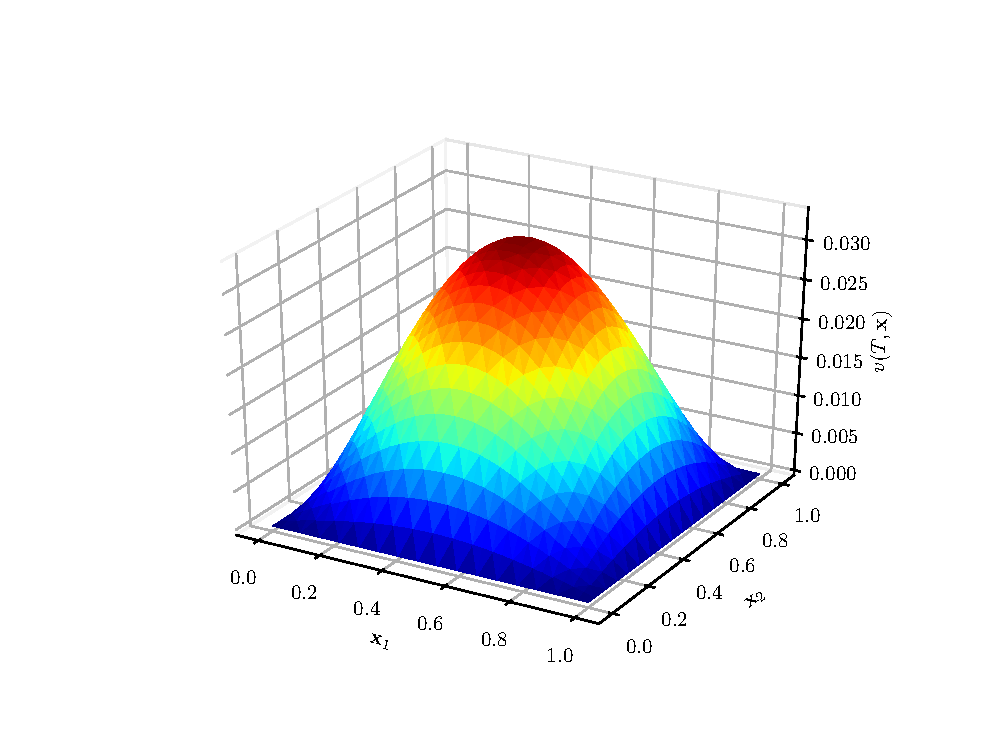
\includegraphics[width=0.8\linewidth]{figures/3d.eps}
  \caption{The solution of the 2D fractional heat equation.}
  \label{fig::md}
\end{figure}
% --------------------------- option pricing results
\subsection{An Application to Option Pricing}
We present numerical results corresponding to the pricing of European call and put options with continuous payoff funtions, and digital options with discontinuous payoffs. In the following, we denote by $(S_t)_{t\ge0}$ the price process of the underlying asset, $K$ the strike price and $T$ the option maturity. The payoff of the option is denoted by $g(s)$, where it is equal to $(s-K)^+$ for call options, $(K-s)^+$ for put options and $\mathbb{1}_{\{s>K\}}$ for digital options. For $\beta = 1/2$ (i.e, $\alpha=1$), the price process follows
\begin{equation} \label{sde_op}
\der S_t = rS_{t^{-}}\der t + \sigma\sqrt{S_{t^{-}}}\der L_t^{1},\quad S_0=s_0, 
\end{equation} 
where $(L_t^{1})_{t\ge 0}$ is an $1$-stable L\'{e}vy process, $r>0$ the risk-free interest rate and $\sigma>0$ the volatility. In this case, existence and uniqueness of solutions to \eqref{sde_op} follow immediately from the conditions discussed previously, with $\kappa(x) = rx$ and $\rho(x) =\sigma \sqrt{x}$. Indeed, $\kappa(x)$ is increasing and concave, $\kappa(0)=0, \int_0^{\infty}rx^{-1}\der x = \infty$ and $|rx-ry| = r|x-y| \le \kappa(|x-y|) \  \forall x,y\in\mathbb{R}.$ In addition to that, we have that $\rho(x)$ is increasing and concave, $\rho(0)=0$ and $\int_0^{\infty}(\sigma\sqrt{x})^{-1}\der x = \infty$. Finally, $|\sigma\sqrt{x}-\sigma\sqrt{y}| = \sigma|\sqrt{x}-\sqrt{y}| \le \sigma \sqrt{|x-y|} = \rho(|x-y|) \ \forall x,y\in\mathbb{R}.$ Indeed and assuming wlog.\ that $x\ge y>0$, squaring both sides of the latter inequality leads to
\begin{equation*}
x-2\sqrt{xy}+y \le x-y \implies 2\sqrt{xy} \ge 2y,
\end{equation*}
which follows from the assumption that $x\ge y.$
The infinitesimal generator $\mathcal{A}^1$ of the process $S$ is 
\begin{equation*}
\mathcal{A}^1 = rs\partial_s - \sigma\sqrt{s}(-\partial_{ss})^{1/2}.
\end{equation*}
The pricing parabolic PDE is then given by 
\begin{equation} \label{pricing_pde}
\begin{split} % \begin{split}
v_t(t,s) + \overbrace{\sigma \sqrt{s}(-\partial_{ss})^{1/2}v(t,s) - rs\partial_sv(t,s)}^{-\mathcal{A}^1v(t,s)} + rv(t,s) = 0&, \quad  (t,s)\in(0,T]\times (0,R), \\
v(0,s) = g(s)&, \quad s\in [0,R], \\ 
v_{\text{Call}}(t,0)=0,\ v_{\text{Digital}}(t,0)=0,\ v_{\text{Put}}(t,R) = 0&, \quad t \in (0,T].
\end{split}
\end{equation}
Call and digital options are approximated by down-and-out barrier options with barrier $H=0$, so that we impose homogeneous Dirichlet boundary conditions at $s=0$. On the other side, put options are approximated by up-and-out barrier options with barrier $H=R$, and so we impose homogeneous Dirichlet boundary conditions at $s=R$. In that case, the Poincar\'{e} inequality still holds since each of \{R\} and \{0\} has positive counting measure, and hence the whole theory of existence and uniqueness of weak solutions holds.\\ In the following, we fix $r=0.06, \sigma=0.6$ and $T=1$.

\begin{figure}[h]
\centering
\begin{subfigure}{0.5\textwidth}
  \centering
  \includegraphics[width=1\linewidth]{figures/pricing/call_modi.eps}
  \caption{$K=7$, European call option.}
  \label{fig:sub1}
\end{subfigure}%
\begin{subfigure}{0.5\textwidth}
  \centering
  \includegraphics[width=\linewidth]{figures/pricing/put_modi.eps}
  \caption{$K= 7$, European put option.}
  \label{fig:sub2}
\end{subfigure} \\
\begin{subfigure}{0.5\textwidth}
  \centering
  \includegraphics[width=1\linewidth]{figures/pricing/digital_modi.eps}
  \caption{$K=10$, European digital option.}
  \label{fig:sub1}
\end{subfigure}%
\caption{The price of European options under Feller--L\'{e}vy models (orange), together with the payoff (blue). For comparison: the corresponding price values in the Black-Scholes market (green).}
\label{fig:sub2}
\end{figure}


\newpage
% ------ Direct and Iterative Solvers Comparison
\subsection{Comparison of Direct and Iterative Solvers}
In this section we present a comparison in terms of computational time of the direct LU-factorization and the two iterative solvers, CGD and PCGD, all applied in case of the fractional heat equation \eqref{frac_heat_1D} and the pricing problem \eqref{pricing_pde}, for different number of mesh nodes $N$.  Table \eqref{table::time} summarizes the results, where the time is in seconds $(s)$. 
\begin{table}[h]
\centering
\begin{subtable}{0.5\textwidth}
  \centering
\begin{tabular}{|l|l|l|l|l|}
\hline
$N$        & 50   & 70    & 100   & 150                \\ \hline
SparseLU & 43.1 & 125.8 & 387.9 & \textgreater{}1000 \\ \hline
CGD      & 10.2 & 34.3 & 134.1 & 675             \\ \hline
PGCD     & 10.9 & 36.1 & 143.5 & 700.5        \\ \hline
\end{tabular}
  \caption{The fractional heat equation. }
  \label{fig:table1}
\end{subtable}%
\begin{subtable}{0.5\textwidth}
  \centering
\begin{tabular}{|l|l|l|l|l|}
\hline
$N$        & 50   & 70    & 80   & 100               \\ \hline
SparseLU & 73.4 & 186.06 & 288.7 & 602.2 \\ \hline
CGD      & 32.2 & 106.2 & 180.2 & 466.5           \\ \hline
PGCD     & 28.01 & 87.53 & 147.7 & 365.2        \\ \hline
\end{tabular}
  \caption{The pricing problem.}
  \label{fig:tabl2}
\end{subtable}%
\caption{Computational time comparison for the LU-factorization, CGD and PCGD.}
\label{table::time}
\end{table}
For the fractional heat equation, the CGD always outperforms the direct LU solver, however the PCGD performs slightly worse than the CGD, but better than the direct LU solver. As for the pricing problem, the CGD also outperforms the direct LU solver and the same goes for the PCGD, but we notice that the preconditioning improves the computational time as opposed to the case of the fractional heat equation. This can be given an intuitive explanation using the following plot.
\begin{figure}[h]
  \centering
  \includegraphics[width=0.5\linewidth]{figures/kappa.eps}
  \caption{Evolution of the condition number $\kappa$ for the case of the fractional heat equation and the pricing problem for N=50 and N=70. The solid lines correspond to the CGD and the dashed lines correspond to the PCGD.}
  \label{fig:kappa}
\end{figure}\\
The condition number of a matrix $\mathbf{X}$, $\kappa(\mathbf{X})$ is defined by
\begin{equation*}
\kappa(\mathbf{X}) = \frac{\sigma_{\text{max}}}{\sigma_{\text{min}}},
\end{equation*}
where $\sigma$ is a singular value of the matrix $\mathbf{X}$. The solid lines in the plot represent the condition number $\kappa(\myexp^{2lk}\stiff+\mass)$ for all $l$ in the sum in equation \eqref{sinc_quad}, where the iterative solver is applied. On the other side, the dashed lines correspond to the condition number after diagonal preconditioning, that is $\kappa(\mathbf{D}^{-1}(\myexp^{2lk}\stiff+\mass))$ where $\mathbf{D}=\text{diag}(\myexp^{2lk}\stiff+\mass)$. The following code shows how to calculate the condition number of a matrix in C++ Eigen.
\begin{lstlisting}[caption={Condition number computation in C++.}] 
double conditionNumber(Eigen::MatrixXd& A){
	Eigen::SVDJacobi<Eigen::MatrixXd> svd(A); 
	Eigen::VectorXd singularValues = svd.singularValues();
	return singularValues(0) / singularValues(singularValues.size()-1); 
}
\end{lstlisting}
Clearly, we do not get any improvement in the condition number after preconditioning in the case of the fractional heat equation, and that is why the PCGD performs worse in that case. More precisely, we do not get faster convergence of the iterative solver while we are adding the computation overhead of the preconditioning. In contrast, we can see from the plot that the condition number decreases after preconditioning in the pricing problem, and that leads to an improvement in the computational time, gaining a faster convergence that is dominating the computation overhead of the preconditioning, and that explain the corresponding results in table \eqref{table::time}.
